\documentclass[notes,11pt, aspectratio=169]{beamer}

\usepackage{pgfpages}
% These slides also contain speaker notes. You can print just the slides,
% just the notes, or both, depending on the setting below. Comment out the want
% you want.
\setbeameroption{hide notes} % Only slide
%\setbeameroption{show only notes} % Only notes
%\setbeameroption{show notes on second screen=right} % Both

\usepackage{helvet}
\usepackage[default]{lato}
\usepackage{array}
\usepackage{tgbonum}

\usepackage{tikz}
\usepackage{verbatim}
\setbeamertemplate{note page}{\pagecolor{yellow!5}\insertnote}
\usetikzlibrary{positioning}
\usetikzlibrary{snakes}
\usetikzlibrary{calc}
\usetikzlibrary{arrows}
\usetikzlibrary{decorations.markings}
\usetikzlibrary{shapes.misc}
\usetikzlibrary{matrix,shapes,arrows,fit,tikzmark}
\usepackage{amsmath}
\usepackage{mathpazo}
\usepackage{hyperref}
\usepackage{lipsum}
\usepackage{multimedia}
\usepackage{graphicx}
\usepackage{multirow}
\usepackage{graphicx}
\usepackage{dcolumn}
\usepackage{bbm}
\newcolumntype{d}[0]{D{.}{.}{5}}

\usepackage{changepage}
\usepackage{appendixnumberbeamer}
\newcommand{\beginbackup}{
   \newcounter{framenumbervorappendix}
   \setcounter{framenumbervorappendix}{\value{framenumber}}
   \setbeamertemplate{footline}
   {
     \leavevmode%
     \hline
     box{%
       \begin{beamercolorbox}[wd=\paperwidth,ht=2.25ex,dp=1ex,right]{footlinecolor}%
%         \insertframenumber  \hspace*{2ex}
       \end{beamercolorbox}}%
     \vskip0pt%
   }
 }
\newcommand{\backupend}{
   \addtocounter{framenumbervorappendix}{-\value{framenumber}}
   \addtocounter{framenumber}{\value{framenumbervorappendix}}
}


\usepackage{graphicx}
\usepackage[space]{grffile}
\usepackage{booktabs}
\newcommand\independent{\protect\mathpalette{\protect\independenT}{\perp}}
\def\independenT#1#2{\mathrel{\rlap{$#1#2$}\mkern2mu{#1#2}}}
\DeclareMathOperator{\Supp}{Supp}

% These are my colors -- there are many like them, but these ones are mine.
\definecolor{blue}{RGB}{0,114,178}
\definecolor{red}{RGB}{213,94,0}
\definecolor{yellow}{RGB}{240,228,66}
\definecolor{green}{RGB}{0,158,115}

\hypersetup{
  colorlinks=false,
  linkbordercolor = {white},
  linkcolor = {blue}
}


%% I use a beige off white for my background
\definecolor{MyBackground}{RGB}{255,253,218}

%% Uncomment this if you want to change the background color to something else
%\setbeamercolor{background canvas}{bg=MyBackground}

%% Change the bg color to adjust your transition slide background color!
\newenvironment{transitionframe}{
  \setbeamercolor{background canvas}{bg=yellow}
  \begin{frame}}{
    \end{frame}
}

\setbeamercolor{frametitle}{fg=blue}
\setbeamercolor{title}{fg=black}
\setbeamertemplate{footline}[frame number]
\setbeamertemplate{navigation symbols}{}
\setbeamertemplate{itemize items}{-}
\setbeamercolor{itemize item}{fg=blue}
\setbeamercolor{itemize subitem}{fg=blue}
\setbeamercolor{enumerate item}{fg=blue}
\setbeamercolor{enumerate subitem}{fg=blue}
\setbeamercolor{button}{bg=MyBackground,fg=blue,}



% If you like road maps, rather than having clutter at the top, have a roadmap show up at the end of each section
% (and after your introduction)
% Uncomment this is if you want the roadmap!
% \AtBeginSection[]
% {
%    \begin{frame}
%        \frametitle{Roadmap of Talk}
%        \tableofcontents[currentsection]
%    \end{frame}
% }
\setbeamercolor{section in toc}{fg=blue}
\setbeamercolor{subsection in toc}{fg=red}
\setbeamersize{text margin left=1em,text margin right=1em}

\newenvironment{wideitemize}{\itemize\addtolength{\itemsep}{10pt}}{\enditemize}

\usepackage{environ}
\NewEnviron{videoframe}[1]{
  \begin{frame}
    \vspace{-8pt}
    \begin{columns}[onlytextwidth, T] % align columns
      \begin{column}{.70\textwidth}
        \begin{minipage}[t][\textheight][t]
          {\dimexpr\textwidth}
          \vspace{8pt}
          \hspace{4pt} {\Large \sc \textcolor{blue}{#1}}
          \vspace{8pt}

          \BODY
        \end{minipage}
      \end{column}%
      \hfill%
      \begin{column}{.38\textwidth}
        \colorbox{green!20}{\begin{minipage}[t][1.2\textheight][t]
            {\dimexpr\textwidth}
            Face goes here
          \end{minipage}}
      \end{column}%
    \end{columns}
  \end{frame}
}

\pgfdeclareimage[height=\paperheight]{mybackground}{images/diff_in_diff.png}


\setbeamertemplate{title page}{

        \begin{picture}(0,0)

            \put(-11,-150){%
                \pgfuseimage{mybackground}
            }

            \put(0,-50.7){%
                \begin{minipage}[b][45mm][t]{226mm}
                    \usebeamerfont{title}{\inserttitle\par}
                \end{minipage}
            }

            \end{picture}

    }


\title[]{\textcolor{blue}{Canonical Research Designs I:\\ Difference-in-Differences:\\ Staggered Timing and Event Studies}}
\author[PGP]{}
\institute[FRBNY]{\small{\begin{tabular}{c}
  Paul Goldsmith-Pinkham  \\
\end{tabular}}}

\date{\today}

\begin{document}

%%% TIKZ STUFF
\tikzset{
	every picture/.style={remember picture,baseline},
	every node/.style={anchor=base,align=center,outer sep=1.5pt},
	every path/.style={thick},
}
\newcommand\marktopleft[1]{%
	\tikz[overlay,remember picture]
	\node (marker-#1-a) at (-.3em,.3em) {};%
}
\newcommand\markbottomright[2]{%
	\tikz[overlay,remember picture]
	\node (marker-#1-b) at (0em,0em) {};%
}
\tikzstyle{every picture}+=[remember picture]
\tikzstyle{mybox} =[draw=black, very thick, rectangle, inner sep=10pt, inner ysep=20pt]
\tikzstyle{fancytitle} =[draw=black,fill=red, text=white]
%%%% END TIKZ STUFF

% Title Slide
\begin{frame}
	\maketitle
\end{frame}

%% Opening example: Yagan (2015) -- single timing, T periods

\begin{frame}{Yagan (2015)}
	\begin{wideitemize}
		\item Yagan (2015) tests whether the 2003 dividend tax cut
		stimulated corporate investment and increased labor earnings
		\item Big empirical question for corporate  finance and public finance
		\item No direct evidence on the real effects of dividend tax cut
		\begin{itemize}
			\item real corporate outcomes are too cyclical to distinguish tax
			      effects from business cycle effects, and economy boomed
		\end{itemize}
		\item Paper uses distinction between ``C'' corp and ``S'' corp designation to estimate effect
		\begin{itemize}
			\item Key feature of law: S-corps didn't have dividend taxation
		\end{itemize}
		\item Identifying assumption (from paper):
		\begin{quote}
			The identifying assumption underlying this research design is
			not random assignment of C- versus S-status; it is that C- and
			S-corporation outcomes would have trended similarly in the
			absence of the tax cut.
		\end{quote}
	\end{wideitemize}
\end{frame}

\begin{frame}{Investment Effects (none)}
	\makebox[\linewidth][c]{
		\resizebox{\linewidth}{!}{
			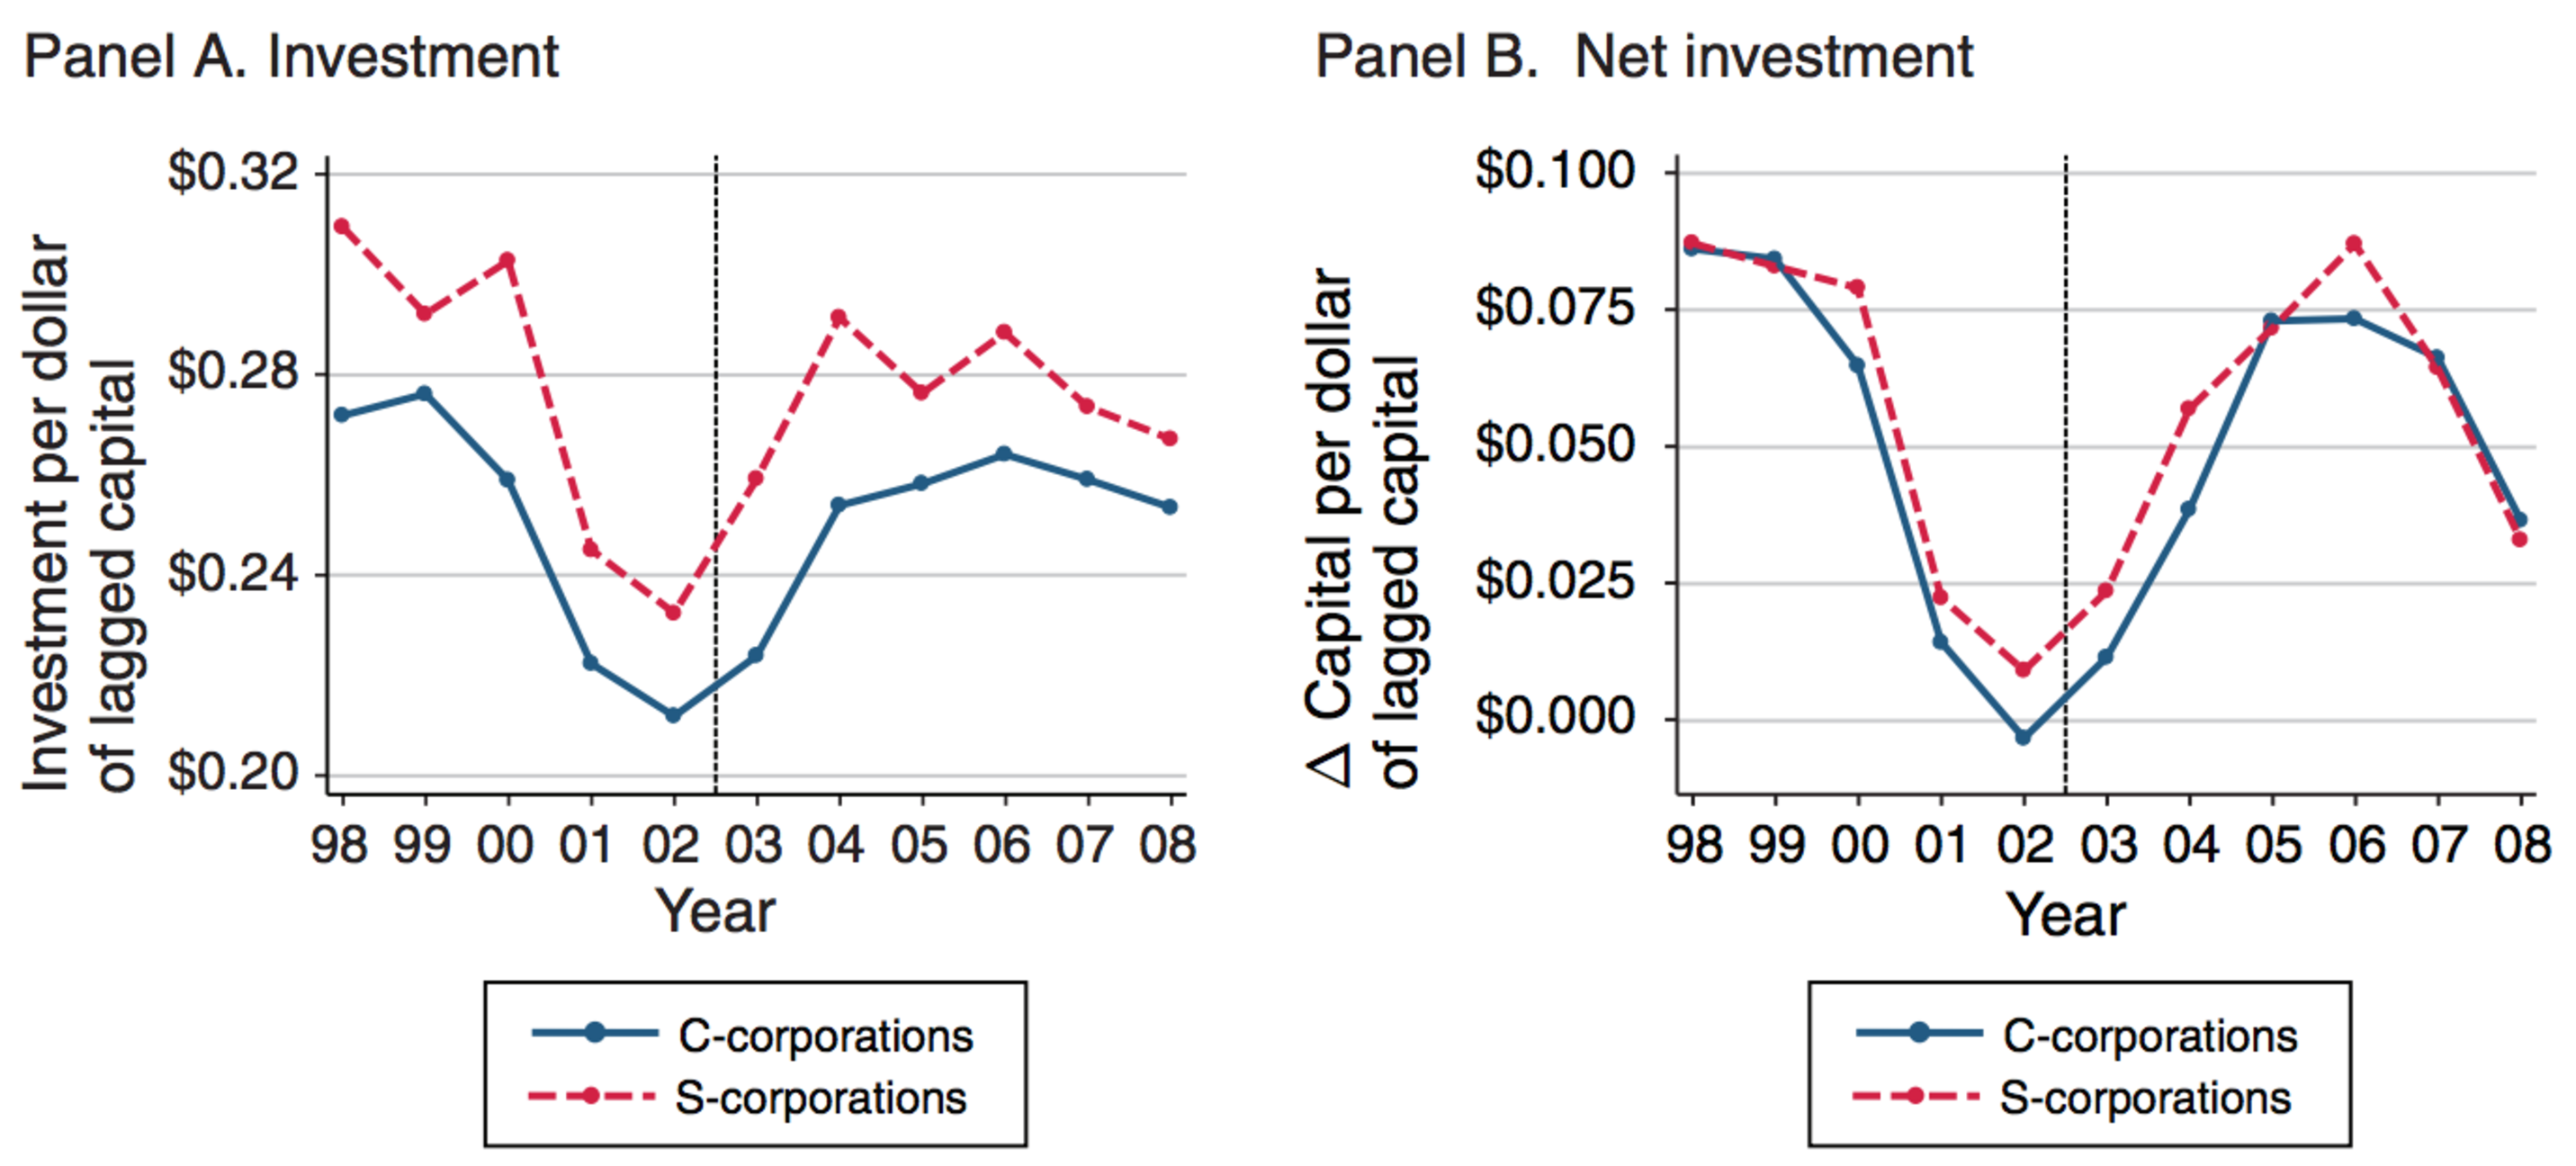
\includegraphics{images/yagan_1.pdf}
		}
	}
\end{frame}
\begin{frame}{Employee + Shareholder effects (big)}
	\makebox[\linewidth][c]{
		\resizebox{\linewidth}{!}{
			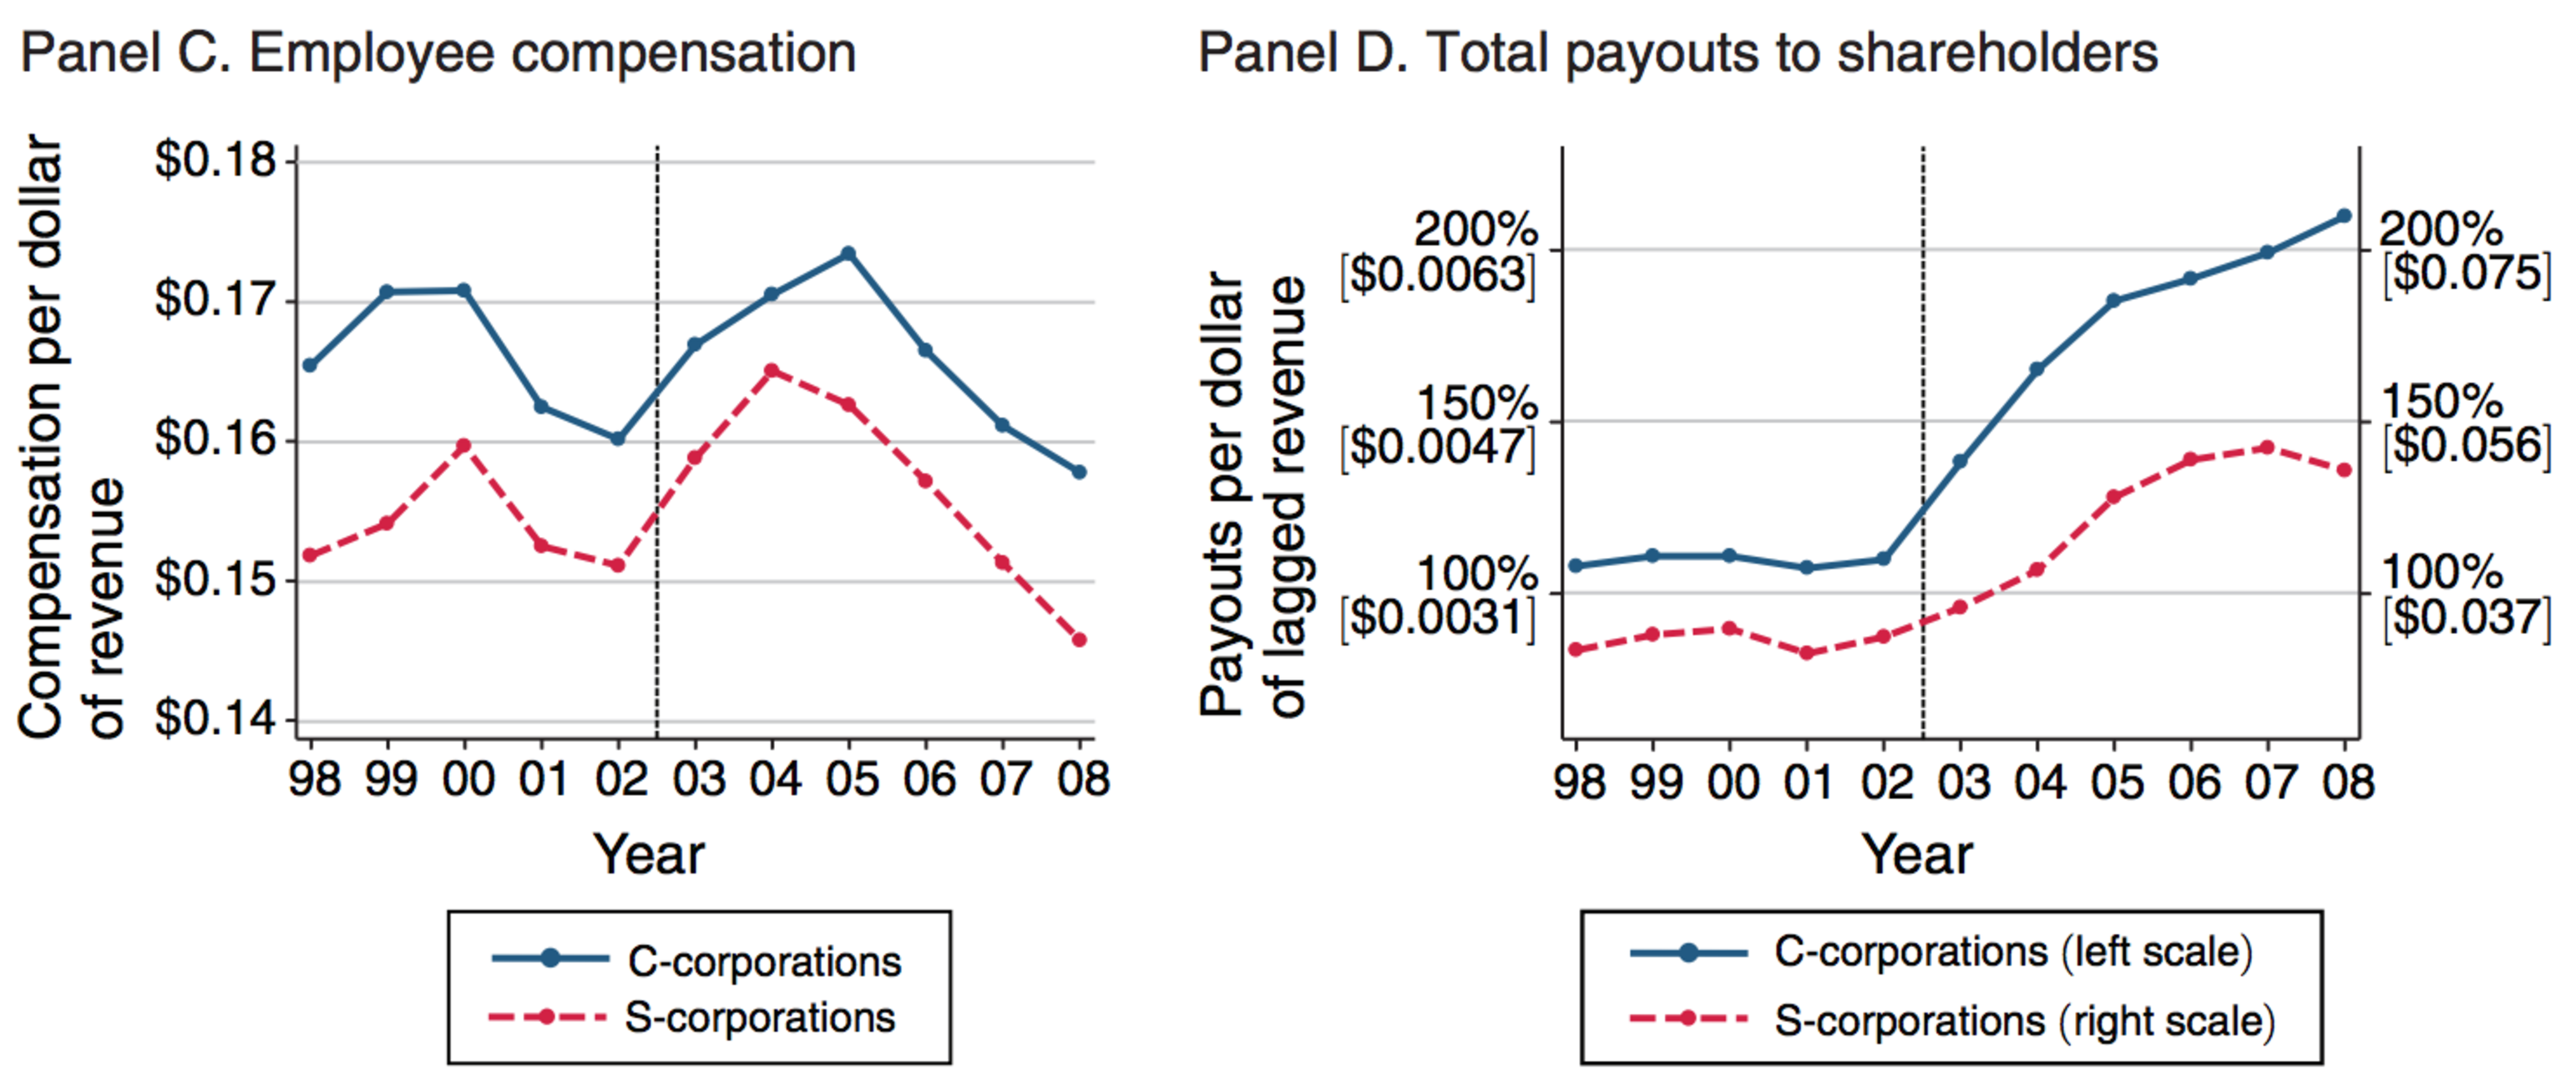
\includegraphics{images/yagan_2.pdf}
		}
	}
\end{frame}

\begin{frame}{Key Takeaway + threats}
	\begin{wideitemize}
		\item Tax reform had zero impact on differential investment and employee compensation
		\item Challenges orthodoxy on estimates of cost-of-capital elasticity of investment
		\item What are underlying challenges to identification?
		\begin{enumerate}
			\item Have to assume (and try to prove) that the only differential
			      effect to S- vs C-corporations was through dividend tax changes
			\item During 2003, could other shocks differentially impact?
			      \begin{itemize}
				      \item Yes, accelerated depreciation -- but Yagan shows it
				            impacts them similarly.
			      \end{itemize}
		\end{enumerate}
		\item Key point: you have to make \emph{more} assumptions to assume
		that zero \textbf{differential} effect on investment implies zero
		\textbf{aggregate} effect.
	\end{wideitemize}
\end{frame}

%% Event Studies block (from 14_synthetic_dind.tex)

\begin{frame}{Event study}
	\begin{columns}[T] % align columns
		\begin{column}{0.6\textwidth}
			\begin{wideitemize}
				\item Two important cases with these staggered timing dind (event studies)
				\begin{itemize}
					\item There exists a never-treated group who is a potential control group
					\item Everyone is treated eventually  (No group is a ``pure control'')
				\end{itemize}
				\item The older approach to estimate this model was:
				\begin{equation*}
					Y_{it} = \alpha_{i} + \gamma_{t} + \sum_{s = L_{0}, s\not=-1}^{L_{1}}1(t-T_{i} = s)\mu_{s}
				\end{equation*}
				\item Without a true control group, can't have both time
				fe, unit fe, and the full set of relative effects
				\vspace{-15pt}
				\item Need to exclude both the baseline period AND at least
				some periods outside the treatment window
			\end{wideitemize}
		\end{column}%
		\hfill%
		\begin{column}{.4\textwidth}
			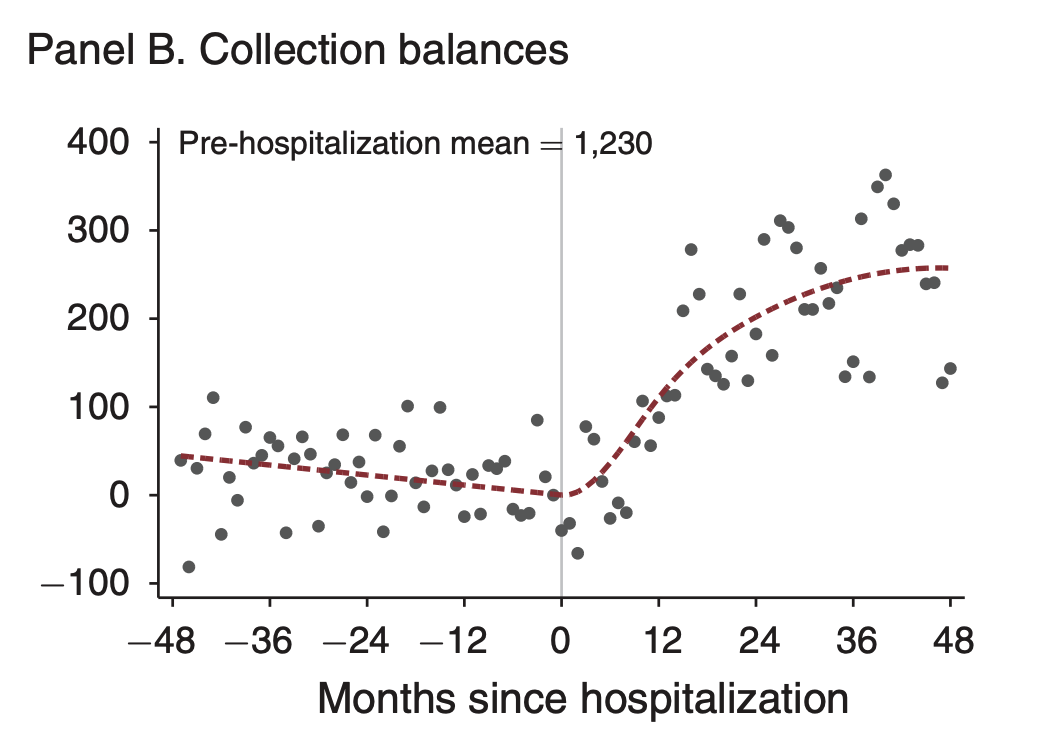
\includegraphics[width=\linewidth]{images/noto1.png}\\
			\begin{itemize}
				\item Dobkin et al. (2018)
				\item Comparison is between those not yet hospitalized and those hospitalized
			\end{itemize}
		\end{column}%
	\end{columns}
\end{frame}

\begin{frame}{Event study continued}
	\begin{wideitemize}
		\item The necessary assumptions are the same (or similar) what we discussed last class
		\item Parallel trends
		\begin{equation}
			E(Y_{i,t}(\infty) - Y_{i,t'}(\infty) | G_{i} = g) =       E(Y_{i,t}(\infty) - Y_{i,t'}(\infty) | G_{i} = g) , \forall g, g', \text{and} t, t'
		\end{equation}
		\item Turns out, all of the groups need to be parallel.
		\item That might be a bad assumption (e.g. very far apart from
		one another)
		\begin{itemize}
			\item Can be weakened in some cases, but only partially
		\end{itemize}
		\item No anticipation:
		\begin{equation}
			Y_{it}(g) = Y_{it}(\infty) \forall t < g
		\end{equation}
	\end{wideitemize}
\end{frame}

\begin{frame}{Contamination Bias in event studies}
	\begin{wideitemize}
		\item Sun and Abraham (2021) show that if the dynamic path of
		treatment is the same across cohorts ($g$), then the coefficient
		from the TWFE model will correctly estimate the period ATT
		$$\tau_{it}(g)  = \sum_{s\geq0}\tau_{s}1(t-g = s)$$
		\item If not, then there is $g$ specific heterogeneity in paths. This creates issues:
		\begin{itemize}
			\item Violate the pre-trend test as the use of ``excluded''
			      periods potentially contaminates pre-periods
			\item Mismeasure the dynamic effects
			\item Additional untestable assumptions are required as we allow for more types of heterogeneity
		\end{itemize}
	\end{wideitemize}
\end{frame}

\begin{frame}{Issues in Diff-in-Diff - Negative Weighting vs. Contamination Bias}
	\begin{wideitemize}
		\item There are two distinct issues in staggered timings:
		\begin{enumerate}
			\item Goodman-Bacon (2021) and others show that the aggregated
			      TWFE estimate can put \emph{negative} weight on some treatment
			      cohorts, thereby giving nonsensical estimands
			\item Sun and Abraham (2021) and others show that the
			      \emph{dynamic} TWFE estimates can be \emph{contaminated} across
			      time
		\end{enumerate}
		\item See discussion in Goldsmith-Pinkham, Hull and Kolesar (2022)
		appendix for analogy to broader linear regression issue
		\item Key point: TWFE linear regression is misspecified
	\end{wideitemize}
\end{frame}

%% Bailey & Goodman-Bacon example (from 13_dind.tex)

\begin{frame}{Bailey and Goodman-Bacon (2015)}
	\begin{wideitemize}
		\item Paper studies  impact of rollout of Community Health Centers on mortality
		\begin{itemize}
			\item Idea is that CHCs can help lower mortality (esp. among
			      elderly) by providing accessible preventative care
		\end{itemize}
		\item Exploit timing of implementation of CHCs
		\begin{quote}
			Our empirical strategy uses variation in when and where CHC
			programs were established to quantify their effects on
			mortality rates. The findings from two empirical tests support
			a key assumption of this approach—that the timing of CHC
			establishment is uncorrelated with other determinants of
			changes in mortality.
		\end{quote}
		\item Issue is that CHCs tend to be done in places
		\item Since CHCs are started in different places in different time
		periods, we estimate effects in \emph{event-time}, e.g. relative
		to initial rollout.
	\end{wideitemize}
\end{frame}

\begin{frame}{Negative effect on mortality}
	\makebox[\linewidth][c]{
		\resizebox{0.7\linewidth}{!}{
			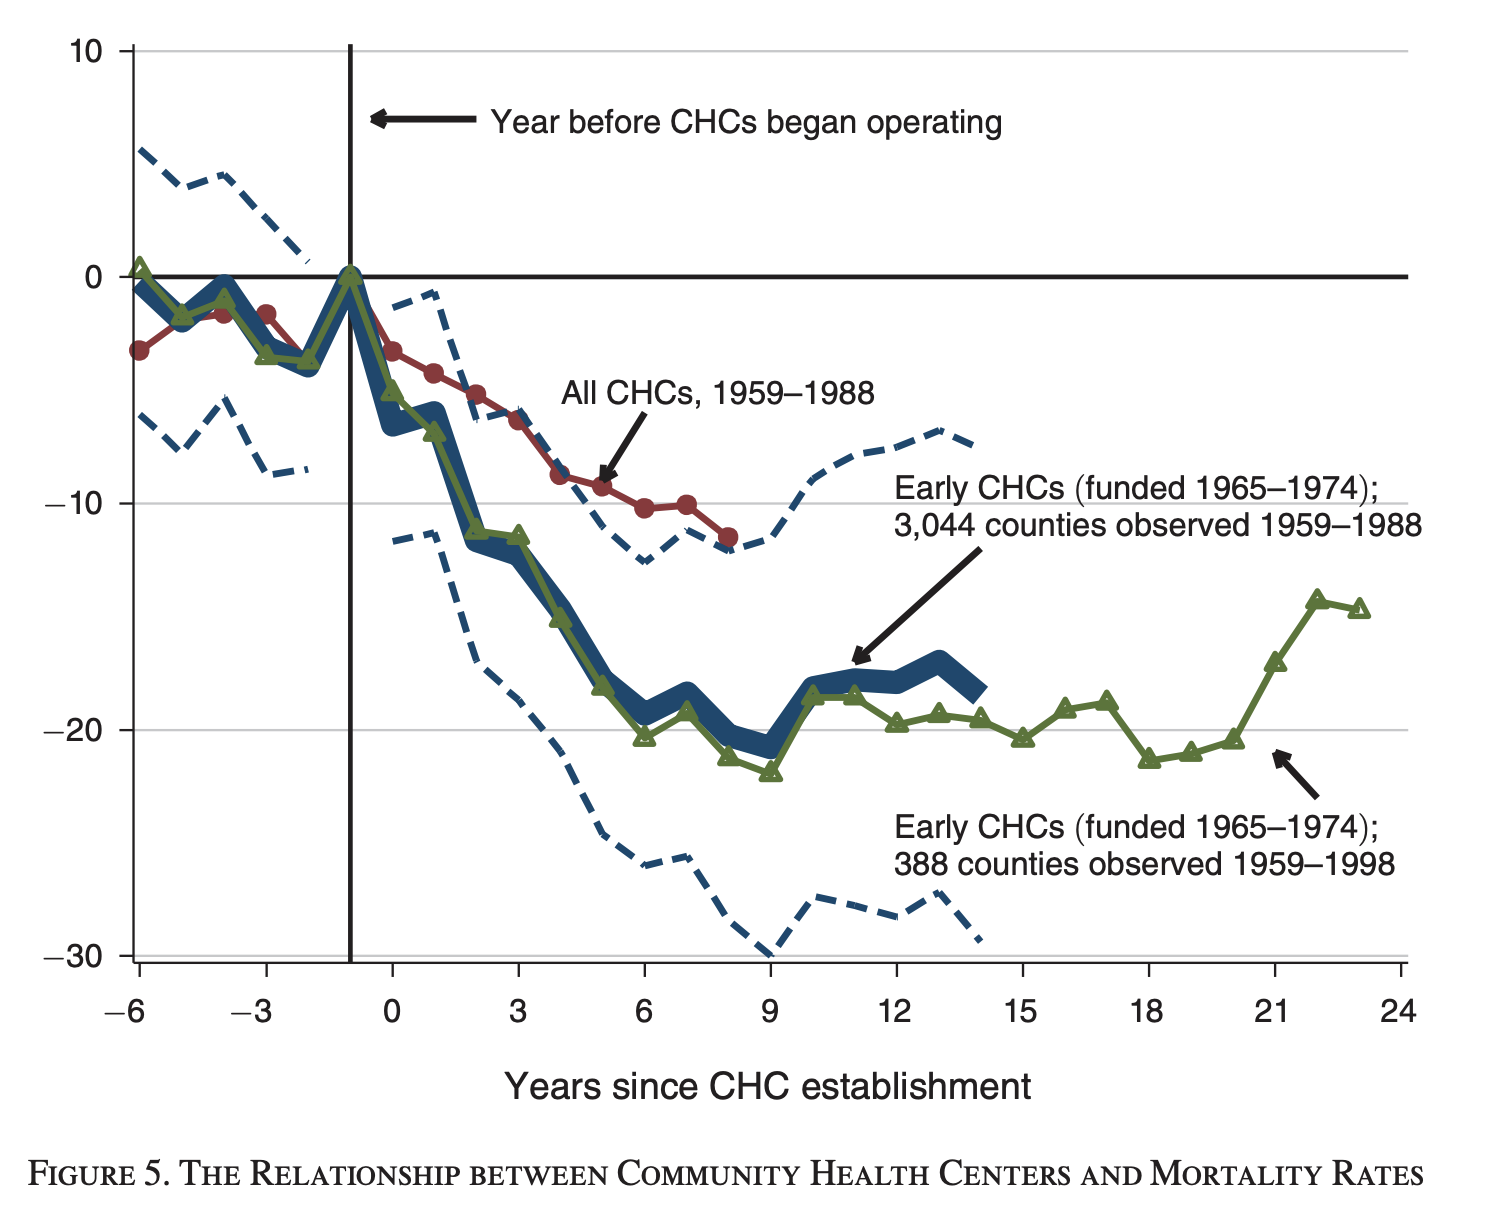
\includegraphics{images/baileygb.png}
		}
	}
\end{frame}
\begin{frame}{Negative effect on mortality, particularly among elderly}
	\makebox[\linewidth][c]{
		\resizebox{0.7\linewidth}{!}{
			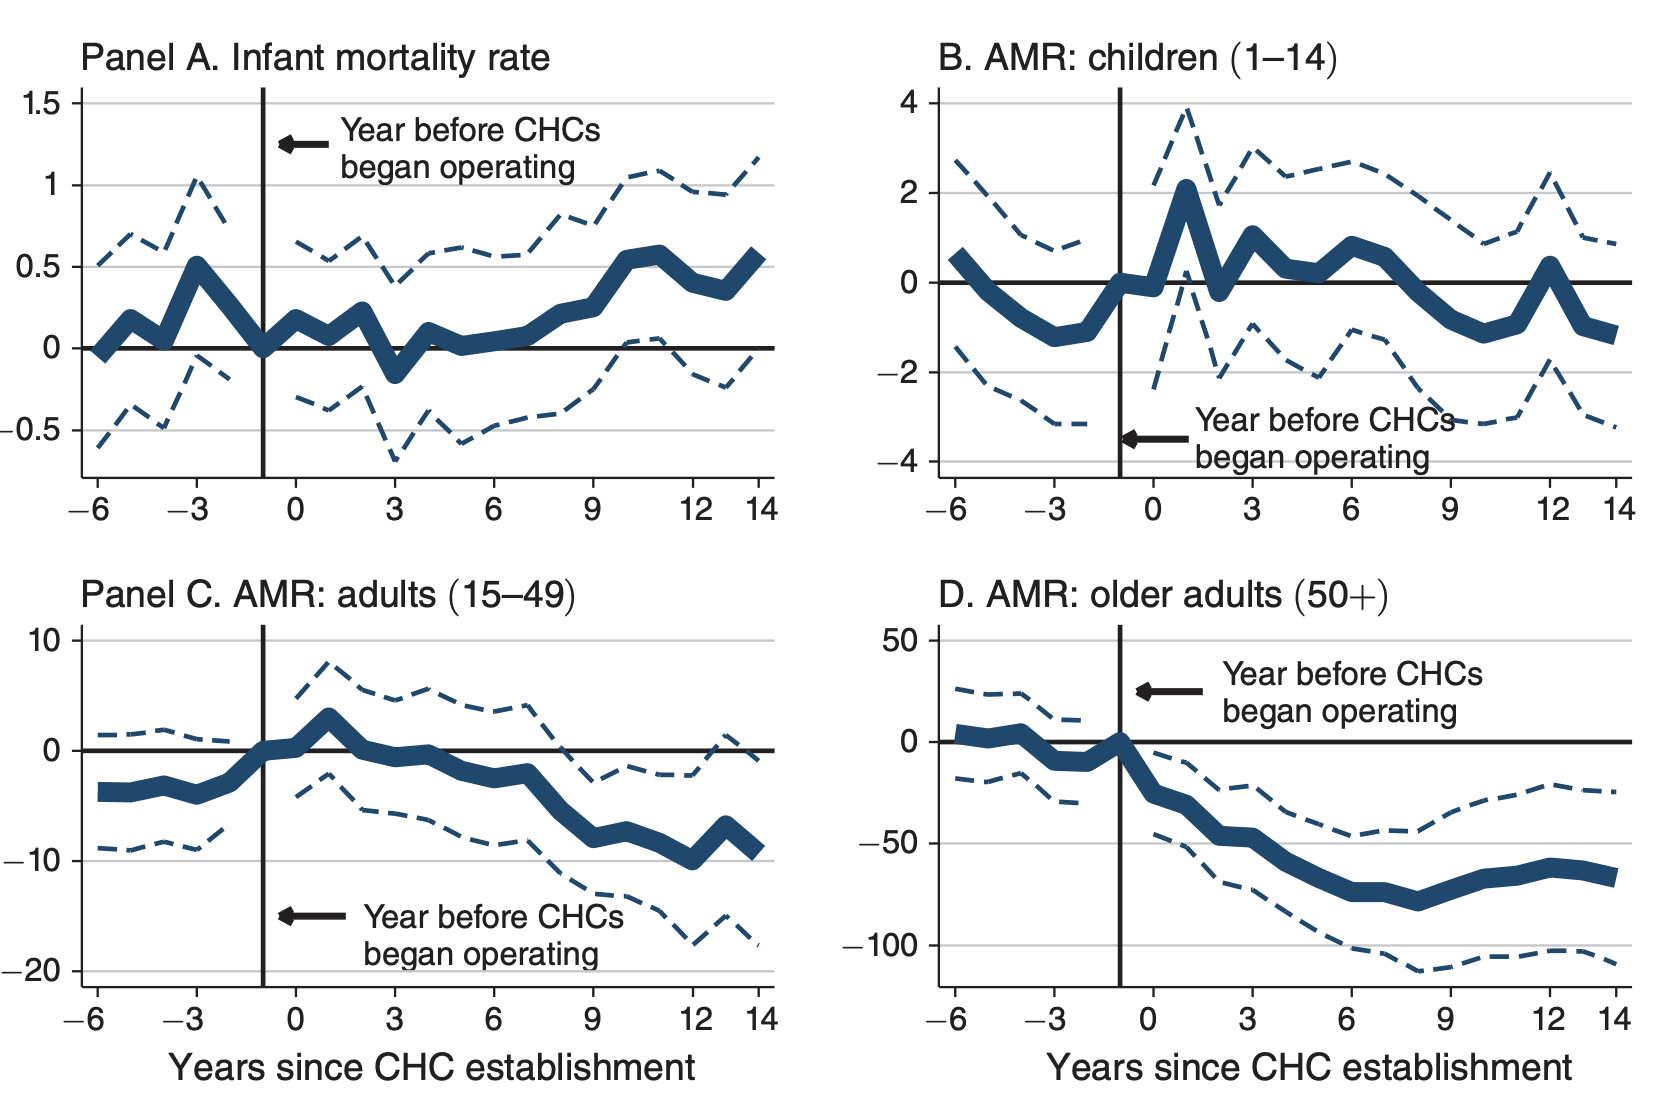
\includegraphics{images/baileygb2.png}
		}
	}
\end{frame}

\begin{frame}{Key takeaways}
	\begin{wideitemize}

		%%% ADD PIECE SHOWING WHY THERE"S POTENTIALLY A PROBLEM WITH ONLY ONE TIME PERIOD
		%%% ADD NOTATION WITH STAGGERED IMPLEMENTATION HERE
		\item Since the policy changes are staggered, we are less worried about effect driven by one confounding macro shock.
		\item Easier to defend story that has effects across different timings
		\begin{itemize}
			\item Also allows us to test for heterogeneity in the time series
		\end{itemize}
		\item Still makes the exact same identifying assumptions -- parallel
		trends in absence of changes
	\end{wideitemize}
\end{frame}

%% TWFE problems with staggered timing (from 13_dind.tex)

\begin{frame}{But a big issue emerges when we exploit differential timing}
	\begin{wideitemize}
		\item We have been extrapolating from the simple pre-post,
		treatment-control setting to broader cases
		\begin{itemize}
			\item multiple time periods of treatment
		\end{itemize}
		\item In fact, in some applications, the policy eventually hits everyone --
		we are just exploiting differential timing.
		\item If we run the ``two-way fixed effects'' model for these times of DinD
		\begin{equation}
			y_{it} = \alpha_{i} + \alpha_{t} + \beta^{DD}D_{it} + \epsilon_{it}
		\end{equation}
		what comparisons are we doing once we have lots of timings?
		\item Key point: is our \emph{estimator} mapping to our \emph{estimand}?
		\item Well, what's our estimand?
	\end{wideitemize}
\end{frame}


\begin{frame}{What is our estimand with staggered timings?}
	\begin{wideitemize}
		\item There are a huge host of papers touching on this question
		\item Callaway and Sant'anna (2020) propose the following building block estimand:
		\begin{equation}
			\tau_{ATT}(g,t) = E(Y_{it}(1) - Y_{it}(0) | D_{it} = 1 \forall t \geq g),
		\end{equation}
		the ATT in period $t$ for those units whose treatment turns on in period $g$.
		\begin{itemize}
			\item In the 2x2 case, this was exactly our effect!
			\item This paper assumes absorbing treatment, but can be weakened in
			      other papers (de Chaisemartin and d'Haultfoeuille (2020) discuss
			      this)
		\end{itemize}
		\item It seems very reasonable that for our overall estimand, we
		want some weighted combinated of these ATTs
		\item Callaway and Sant'anna (2020) highlight two ways to identify the above estimand:
		\begin{enumerate}
			\item Parallel trends of treatment group with a group that is ``never-treated'',  $G_{i} = \infty$
			\item Parallel trends of treatment group with the group of the ``not yet treated'',   $G_{i} \geq t + 1$
		\end{enumerate}
		\item Using these estimands, C\&S provide a very natural set of
		potential ways to aggregate these estimands up
	\end{wideitemize}

\end{frame}

\begin{frame}{Wait what happened to TWFE?}
	\begin{wideitemize}
		\item It turns out that the logic of the TWFE does not naturally extend to differential timings
		\begin{itemize}
			\item Recall that from our discussion of linear regression, regression is great because it does a variance weighted approximation:
			      \begin{equation*}
				      \tau = \frac{E(\sigma^{2}_{D}(W_{i})\tau(W_{i}))}{E(\sigma^{2}_{D}(W_{i}))}, \qquad \sigma^{2}_{D}(W_{i}) = E((D_{i} - E(D_{i}|W_{i}))^{2} | W_{i})
			      \end{equation*}
			\item It turns out that in the panel setting with staggered timings,
			      these weights are not necessarily positive
		\end{itemize}
		\item Why? The predicted value of $D_{i,t}$, $\hat{D}_{it}$, may be
		greater than 1 because $E(D_{i}|W_{i})$ is the model is incorrectly specified by
		the two-way fixed effects:
		\begin{equation*}
			\hat{\beta}_{post} = \frac{\sum_{i,t}(D_{it}- \hat{D}_{i,t})Y_{i,t}}{\sum_{i,t}(D_{it}- \hat{D}_{i,t})^{2}}
		\end{equation*}
	\end{wideitemize}
\end{frame}



\begin{frame}{Misspecification in conditional expectation}
	\begin{wideitemize}
		\item An example from GPHK (2022): Three time periods, and three
		groups of units: treated early in period 2 ($n_{E}$), treated late in period 3
		($n_{L}$), and never ($n_{N}$)
		\item The weights in the estimands on the treatment effects will be
		\begin{align}
			\lambda(j,t=3) & = \frac{n_{E} + 2n_{N}}{\kappa}, j \in L \\
			\lambda(j,t=2) & = \frac{n_{N} + 2n_{L}}{\kappa}, j \in E \\
			\lambda(j,t=3) & = \frac{n_{N} - n_{L}}{\kappa}, j \in E,
		\end{align}
		$\kappa$ just scaling. Hence, first two always get positive weight, but the ATT from period 3 of the early adopters is negative if the never-adopters is small relative to late adopters
		\item Key insight from several papers: with staggered timings +
		heterogeneous effects, the TWFE approach to DinD can put negative
		weight on certain groups' TE
		\begin{itemize}
			\item Serious issue for interpretability
		\end{itemize}
		\item This is \emph{solveable}. Merely a construct of being overly
		casual with estimator definition
	\end{wideitemize}
\end{frame}

\begin{frame}{Goodman-Bacon 2x2 comparisons}
	\begin{columns}[T] % align columns
		\begin{column}{0.4\textwidth}
			\begin{wideitemize}
				\item  Consider two staggered treatments and a never-treated group
				\item What does the TWFE estimator estimate?
			\end{wideitemize}
		\end{column}%
		\hfill%
		\begin{column}{.6\textwidth}
			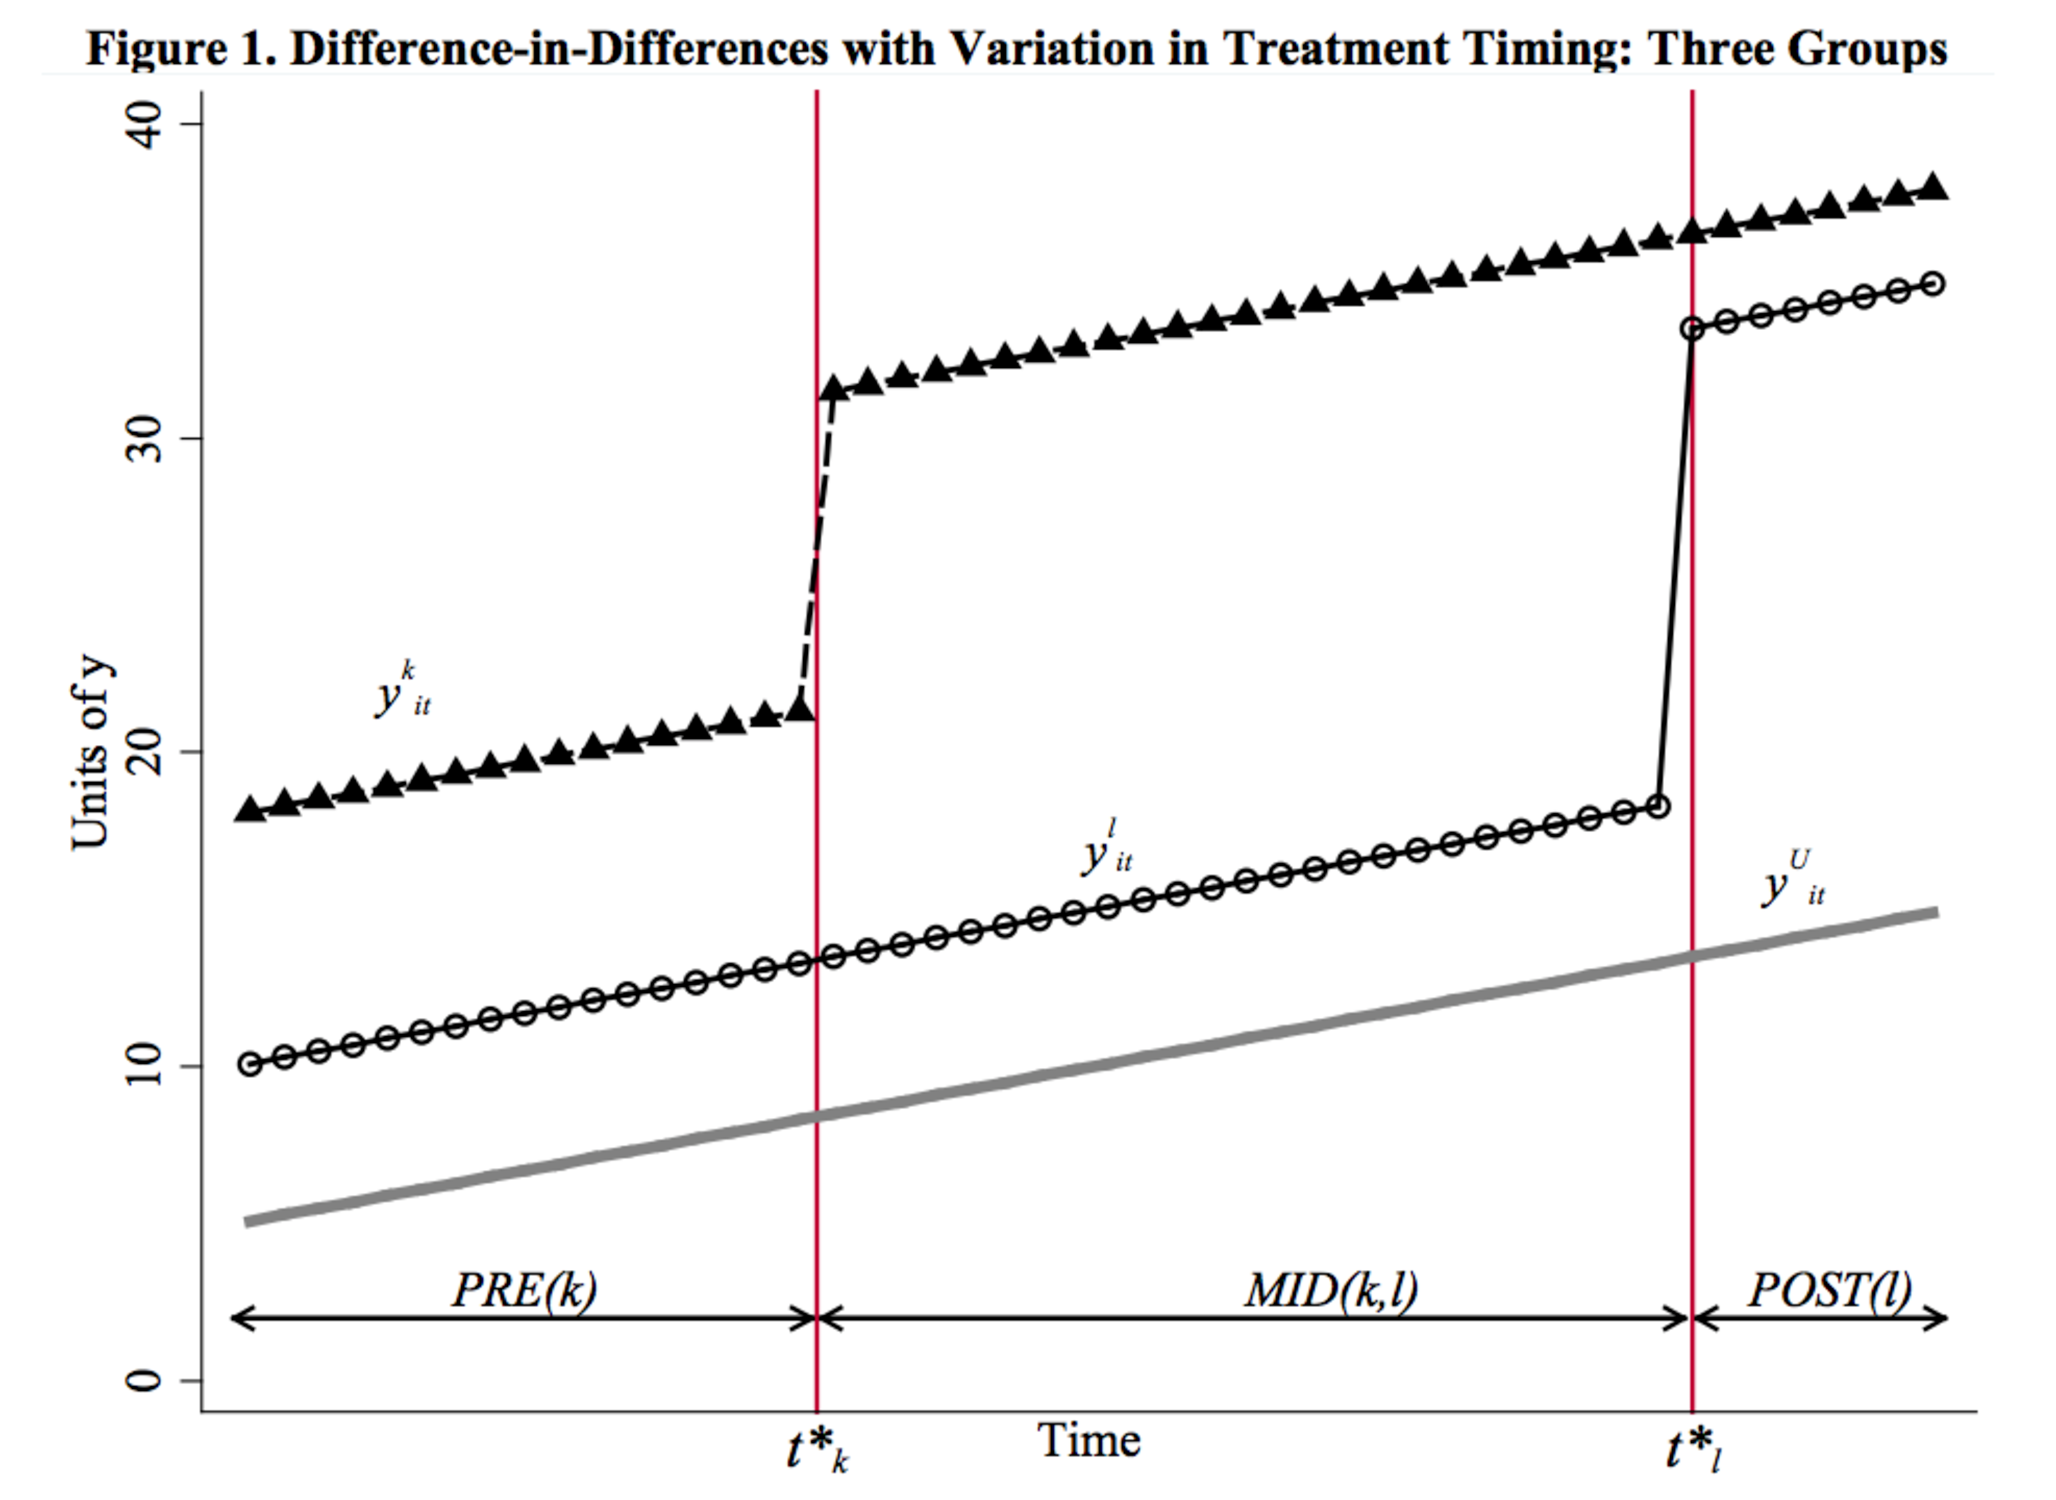
\includegraphics[width=\linewidth]{images/bacon_1.pdf}
		\end{column}%
	\end{columns}
\end{frame}
\begin{frame}{Goodman-Bacon 2x2 comparisons}
	\begin{columns}[T] % align columns
		\begin{column}{0.4\textwidth}
			\begin{wideitemize}
				\item Four potential comparisons that can be made
				\item turns out that TWFE DD estimator (pooled) is the
				weighted average of all 2x2 comparisons
				\item These weights end up putting a high degree of weight on
				units treated in the middle of the sample (since they have the
				highest variance in the treatment indicator!)
			\end{wideitemize}
		\end{column}%
		\hfill%
		\begin{column}{.6\textwidth}
			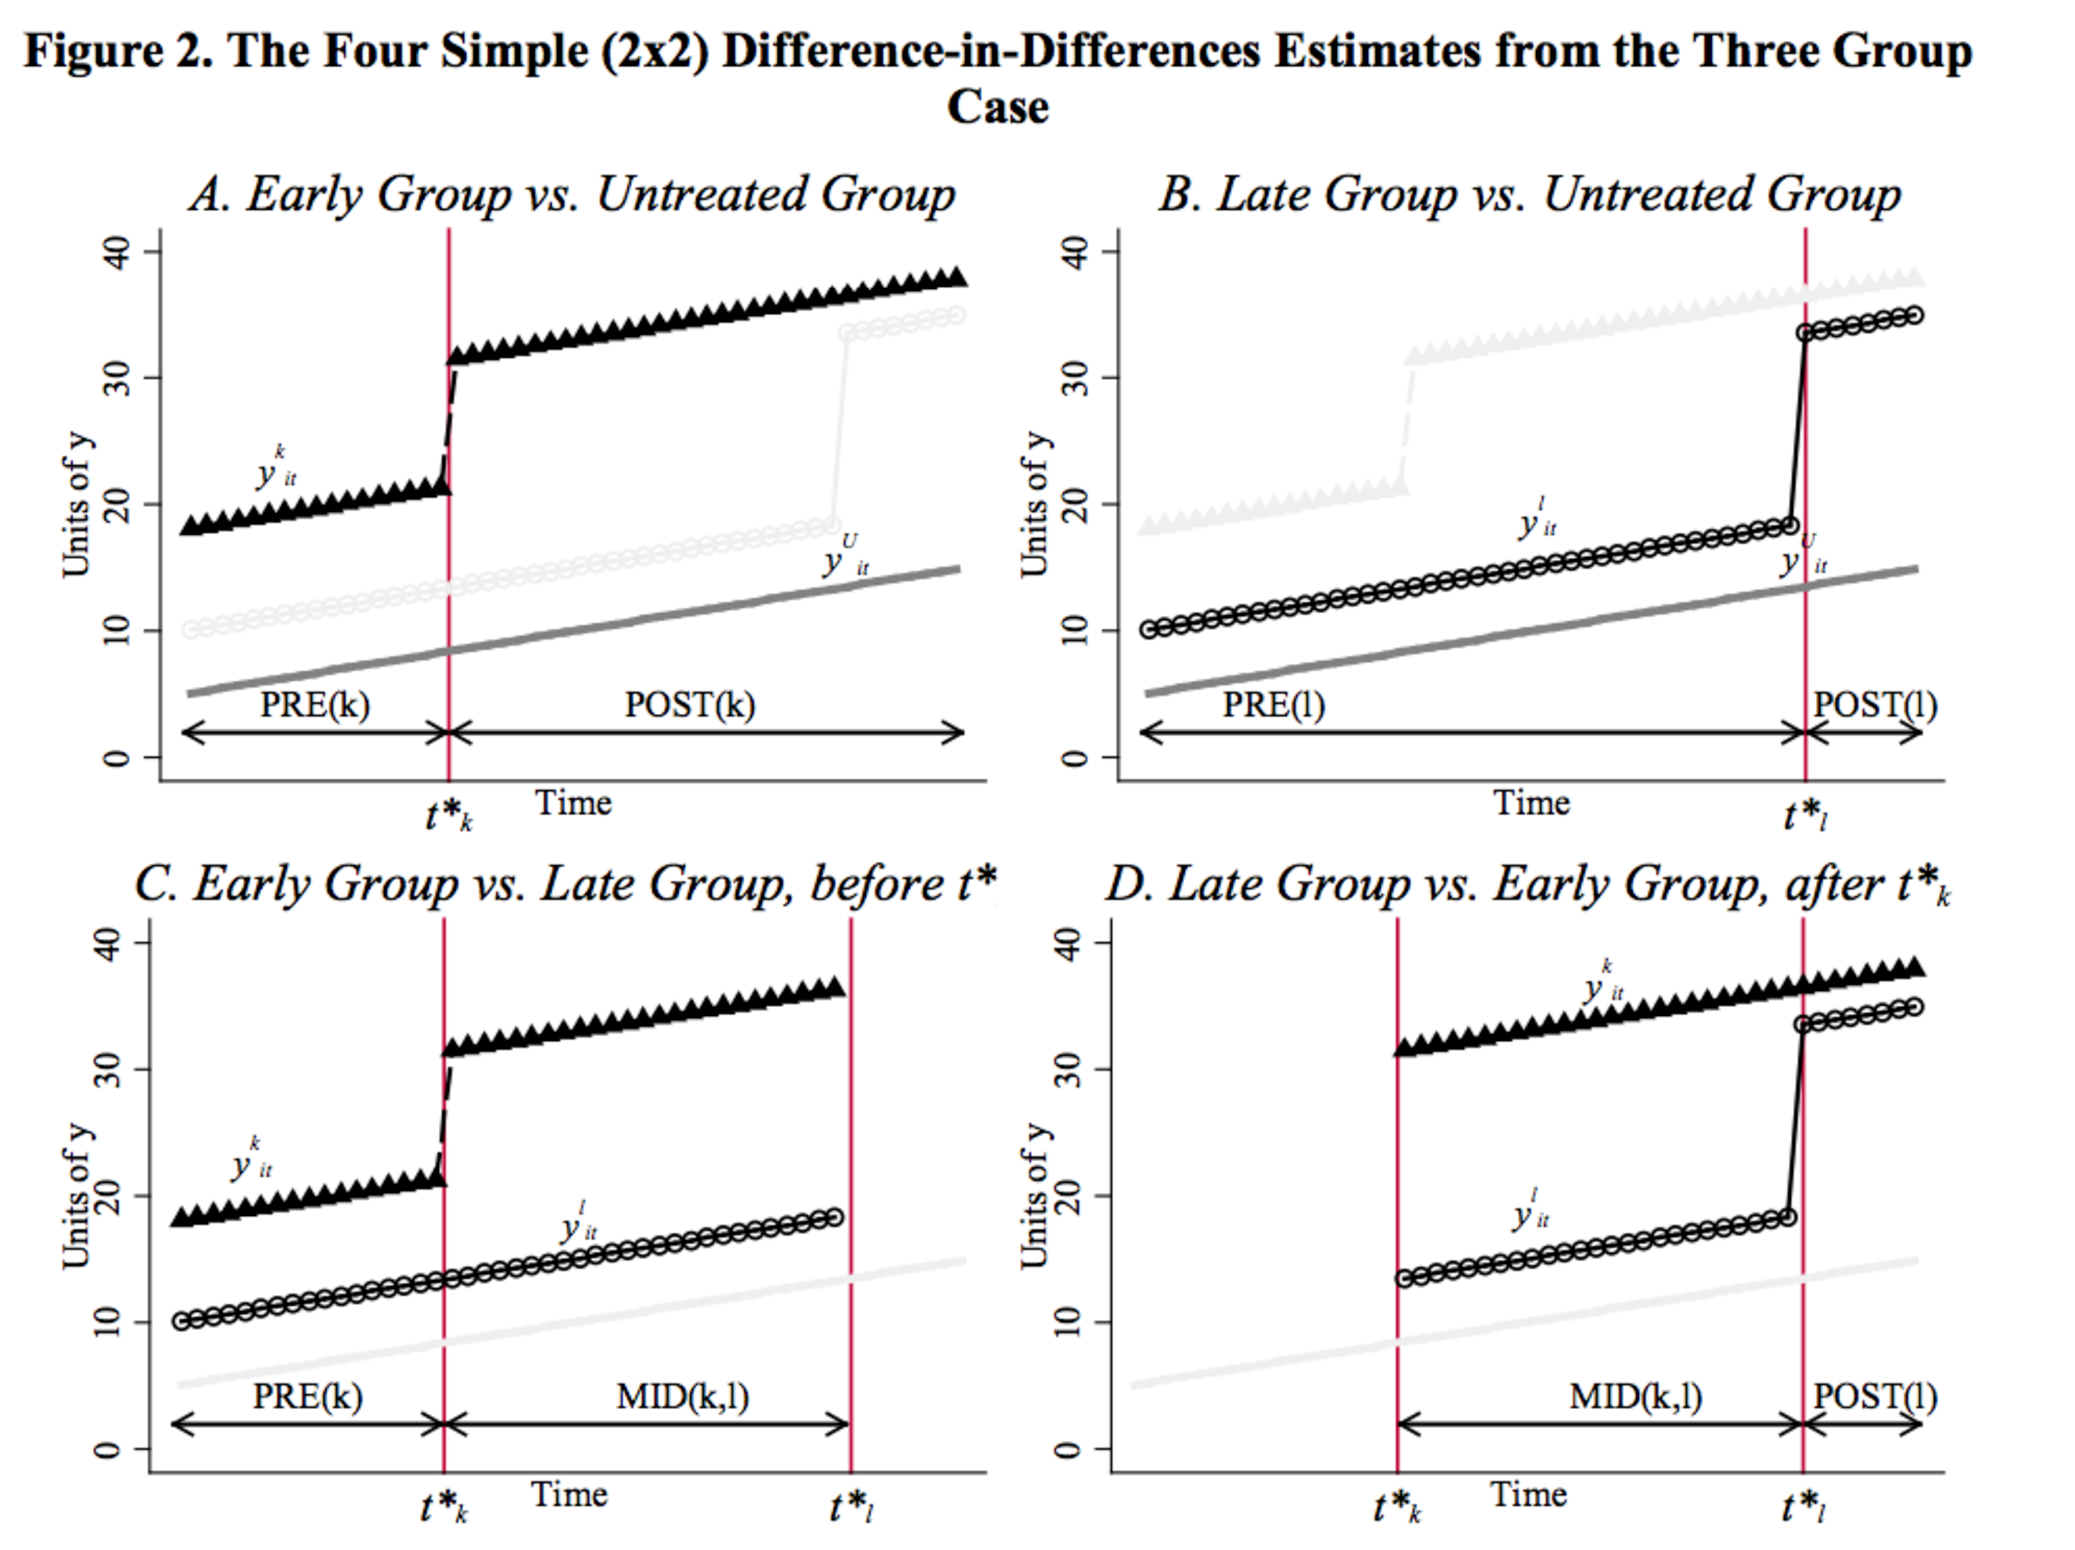
\includegraphics[width=\linewidth]{images/bacon_2.pdf}
		\end{column}%
	\end{columns}
\end{frame}

\begin{frame}{Goodman-Bacon 2x2 comparisons}
	\begin{columns}[T] % align columns
		\begin{column}{0.4\textwidth}
			\begin{wideitemize}
				\item<1-> The weighting becomes problematic if the effects vary
				over time -- if the effects are instantaneous and
				time-invariant, the weights are all positive
				\item<2-> However, time-varying effects create bad
				counterfactual groups, and create negative weights
				\item<2-> Goodman-Bacon provides a way to assess the weights in
				a given TWFE design
			\end{wideitemize}
		\end{column}%
		\hfill%
		\begin{column}{.6\textwidth}
			\only<1>{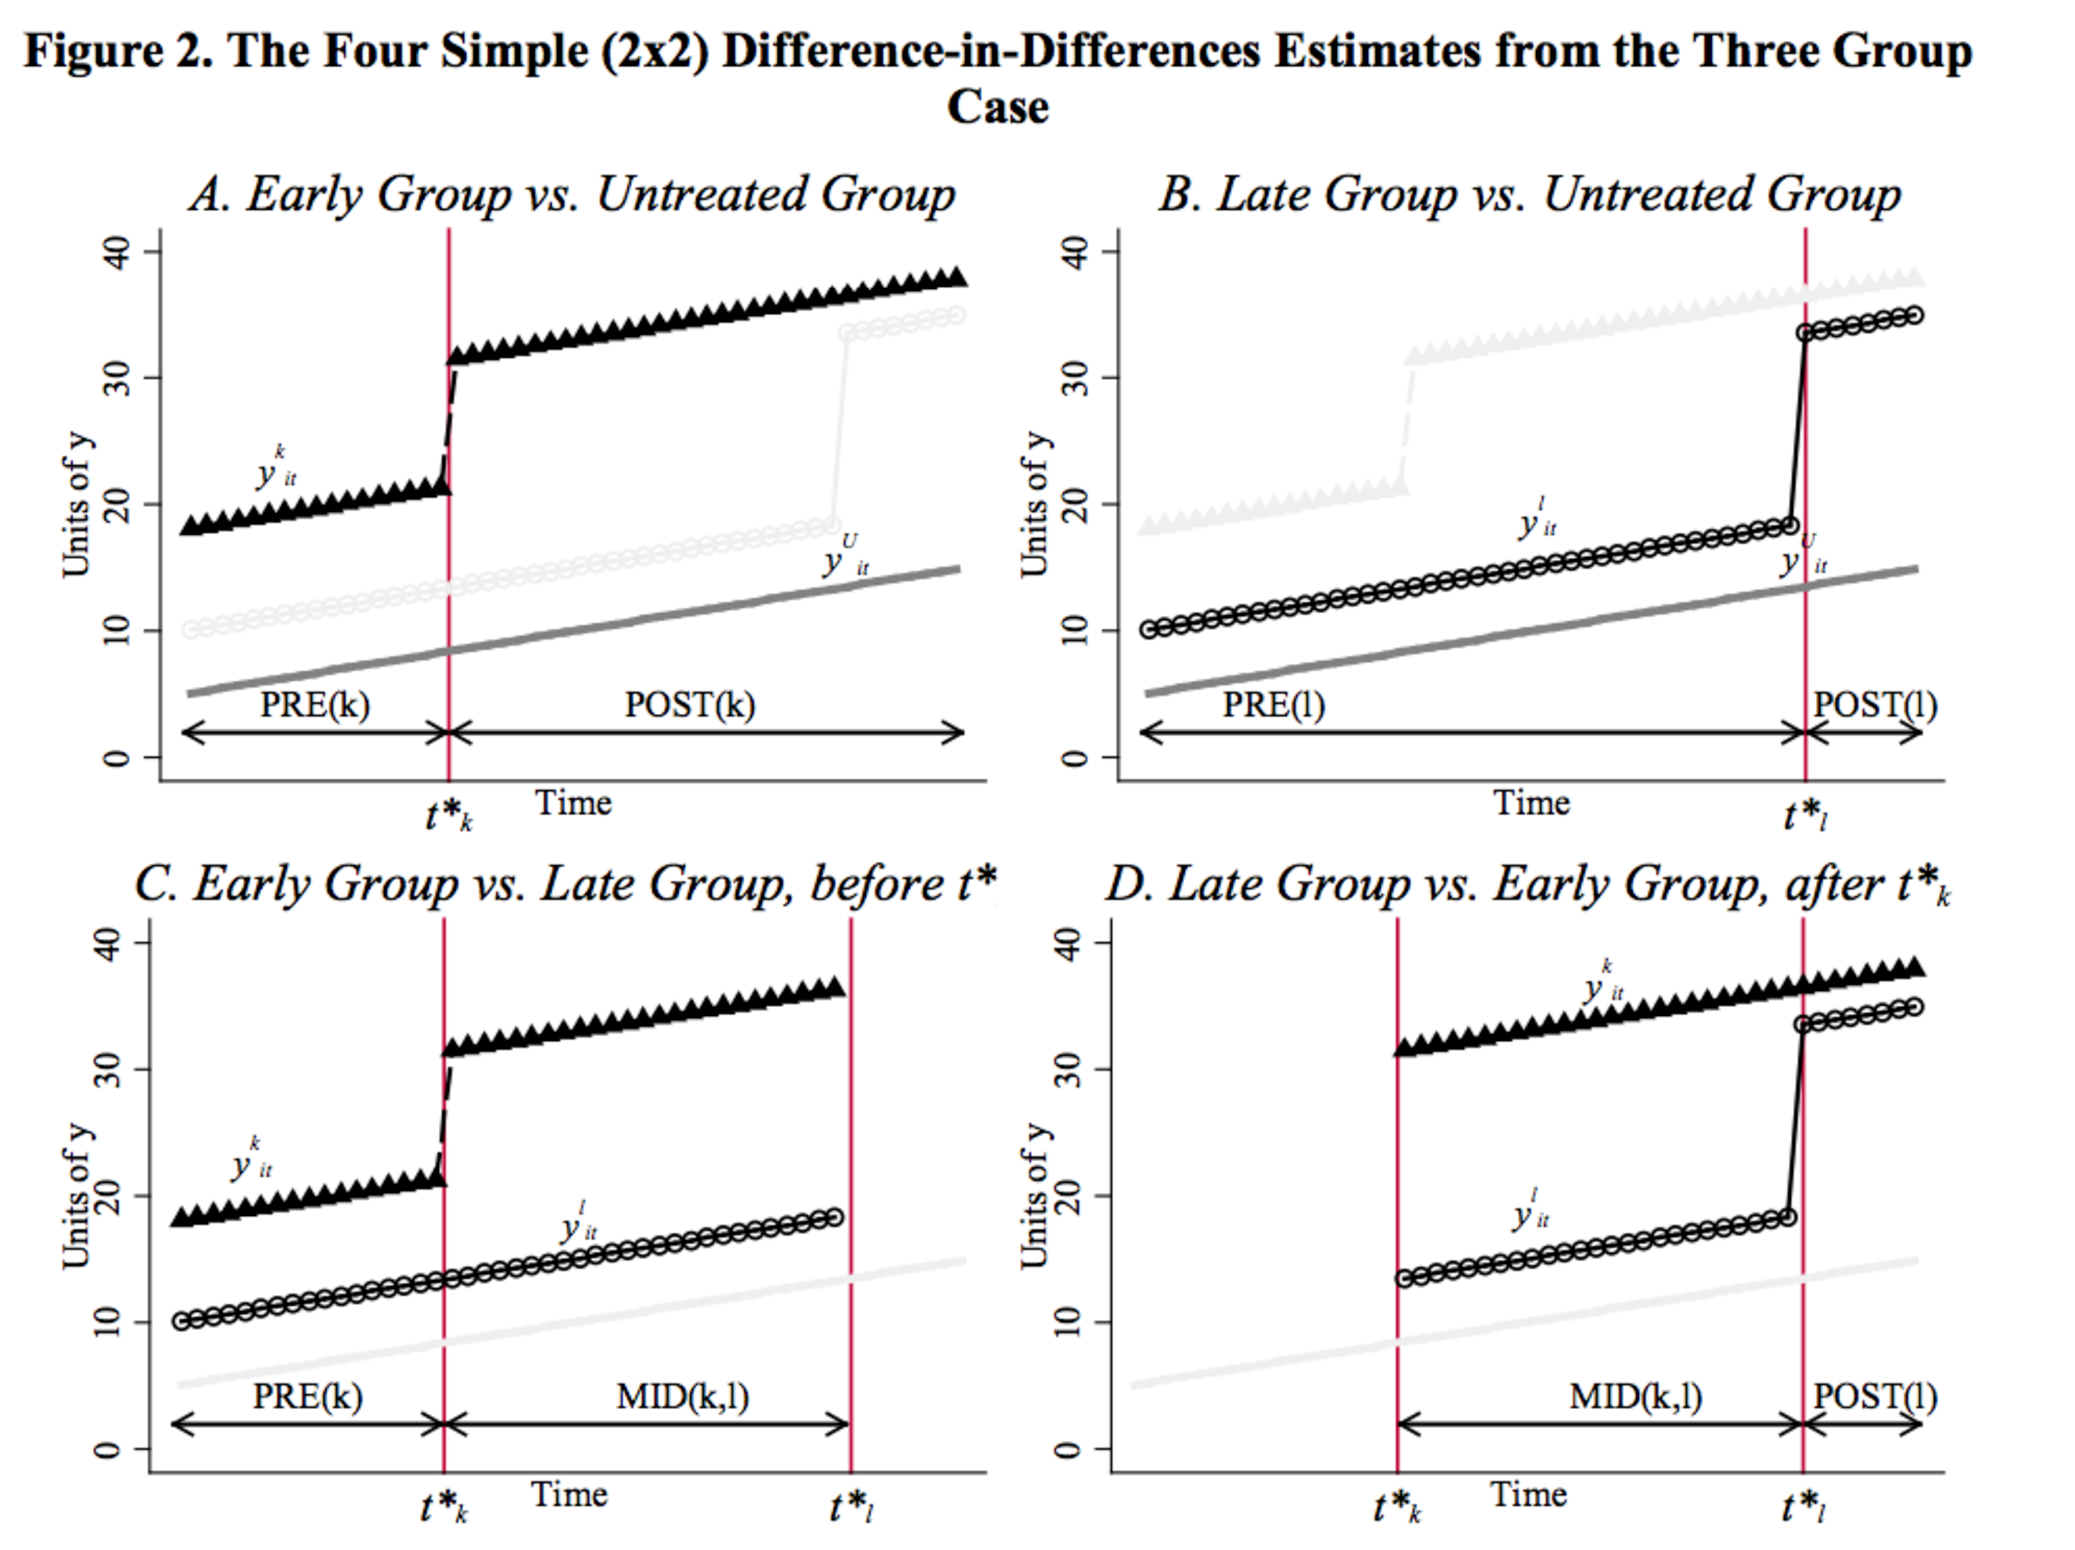
\includegraphics[width=\linewidth]{images/bacon_2.pdf}}
			\only<2>{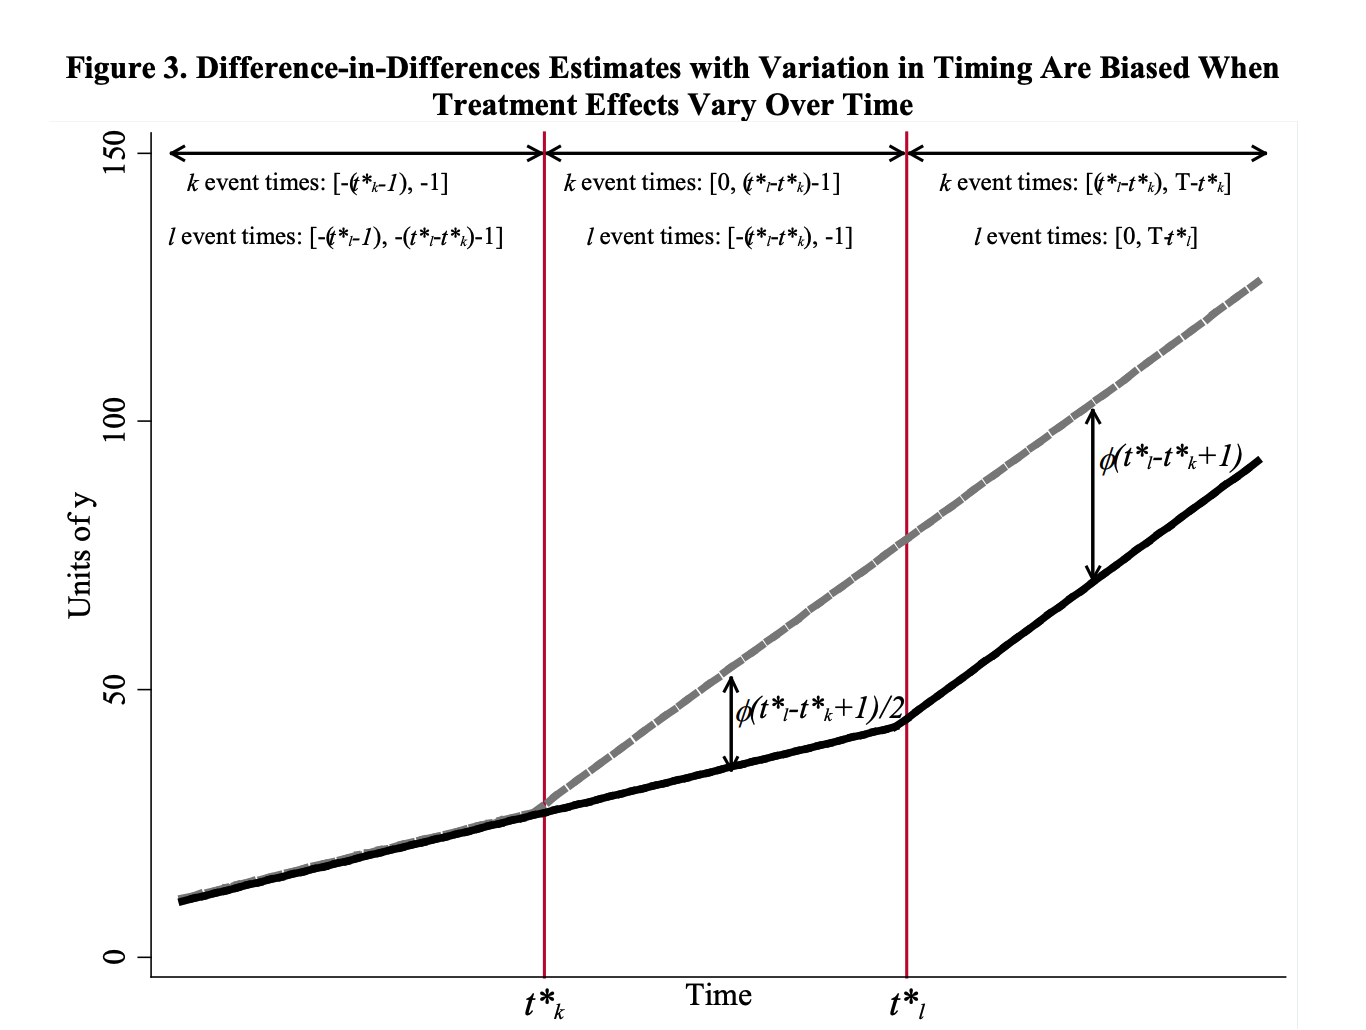
\includegraphics[width=\linewidth]{images/bacon_3.png}}
		\end{column}%
	\end{columns}
\end{frame}

%% Solutions (from 13_dind.tex + 14_synthetic_dind.tex)

\begin{frame}{What to do with staggered timing in DinD?}
	\begin{wideitemize}
		\item There's really no reason to use the baseline TWFE in staggered timings
		\begin{itemize}
			\item A perfect example wherein the estimator does not generate an
			      estimate that maps to a meaningful estimand
		\end{itemize}
		\item There are different approaches proposed in the literature that are just as good!
		\begin{itemize}
			\item E.g. de Chaisemartin and  d'Haultfoeuille (2020), Callaway and Sant'anna (2020)
		\end{itemize}
		\item These all are robust to this issue. I find Callaway and
		Sant'anna quite intuitive, but your circumstances may vary
		slightly. Key piece to keep in mind that differs a bit:
		\begin{itemize}
			\item Is my treatment absorbing?
		\end{itemize}
		\item Irrespective of the exact paper, the key point is that we are
		generating a counterfactual and need to be careful that our
		estimator does so correctly
	\end{wideitemize}
\end{frame}

\begin{frame}{Solutions: Borusyak Hull and Jaravel (2022) Estimator}
	\begin{wideitemize}
		\item Will walk through Sun and Abraham (2021) solution on homework (interacting treatment effects by cohort)
		\item Callaway and Sant'anna (2021) also provided straightforward solution (not using regression)
		\item BHJ impute the counterfactual using the not-yet-treated observations
		\begin{equation}
			Y_{it}(\infty) = \alpha_{i} + \lambda_{t} + \epsilon_{it}
		\end{equation}
		\item Then, we can predict the value for any unit in a time period:
		$\hat{Y}_{i,t}(\infty)$ and proceed accordingly to construct
		measures of group by time period ATT
		($\mu_{ATT}(g,t) = E( Y_{i,t}(g) - \hat{Y}_{i,t}(\infty) | G_{i} =
			g)$
		\item What is key difference from Callaway and Sant'anna (and why it is more efficient under some settings?)
		\begin{itemize}
			\item Estimation of $\alpha_{i}$ uses all the pre-treatment data, rather than just the period before
		\end{itemize}
	\end{wideitemize}
\end{frame}


\begin{frame}{Aside in event studies}
	\begin{columns}[T] % align columns
		\begin{column}{0.5\textwidth}
			\begin{wideitemize}
				\item A key factor in how you construct your counterfactual (and
				what assumptions you find plausible) are a function of how far
				into the future you want to estimate outcomes
				\item An extremely short-run counterfactual could potentially just be a linear extrapolation
				\begin{itemize}
					\item This assumes that the underlying model is locally linear,
					      rather than globally
					\item Construct a counterfactual from just
					      a single time series, but highly non-robust
				\end{itemize}
				\item Example from a robustness check in my own work (Dobbie et al. 2020)
			\end{wideitemize}
		\end{column}%
		\hfill%
		\begin{column}{.5\textwidth}
			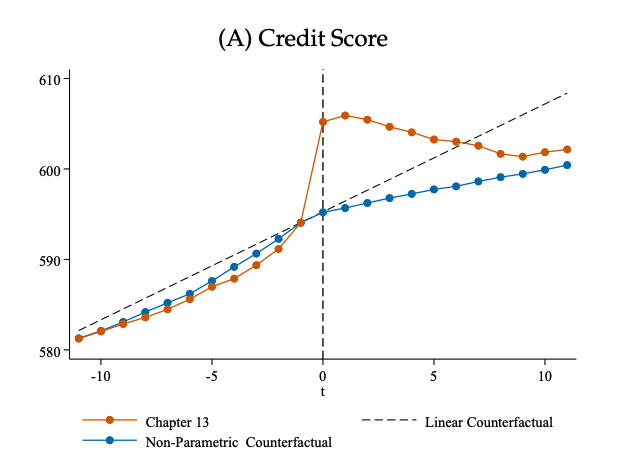
\includegraphics[width=\linewidth]{images/badcredit3.png}
		\end{column}%
	\end{columns}
\end{frame}

\begin{frame}{Constructing a counterfactual is the key goal}
	\begin{wideitemize}
		\item Issue in event study was the attempt to get a ``free lunch''
		-- we always need a control group
		\item   Think back to cross-sectional setting with ATT
		\begin{itemize}
			\item We always knew $Y_{i}(1)$. Key issue is an estimator for $Y_{i}(0)$.
			\item Event study approaches had issues by ignoring this point and hoping regression would solve problem
			\item Notably, this problem disappears if we have full homogeneity + no anticipation and only exclude pre-periods
		\end{itemize}
		\item Point of emphasis -- we need parallel trends to hold to
		construct a counterfactual in these settings. Why?
		$Y_{jt}(0) - Y_{j,t-1}(0)$ needs to be a good approximator of
		$Y_{i,t}(0) - Y_{i,t-1}(0)$.
		\begin{itemize}
			\item Since we imposed
			      $Y_{it} = \alpha_{i} + \gamma_{t} + D_{it}\tau$, the first
			      differencing makes them good approximations
		\end{itemize}
	\end{wideitemize}
\end{frame}

\begin{frame}{Takeaways}
	\begin{wideitemize}
		\item Staggered timing creates real problems for naive TWFE estimation
		\item Two distinct issues: negative weights on treatment effects (Goodman-Bacon) and contamination bias in dynamic specifications (Sun and Abraham)
		\item Solutions exist and are easy to implement: Callaway and Sant'Anna, BHJ imputation, Sun and Abraham interaction-weighted estimator
		\item The core insight: always think carefully about what counterfactual you are constructing
		\item Next class: synthetic control, extensions, and a practitioner's checklist
	\end{wideitemize}
\end{frame}

\end{document}
